\documentclass[final,fmstyle]{./util/ucathesis}
% La opcion 'final' muestra los graficos, para generar una version sin los graficos utiliza la opcion 'draft'

% paquetes recomendados
%\usepackage[chapter]{theorems}
%\usepackage{symbols}
%\usepackage{url}
\usepackage{amsmath,amsthm}

\usepackage[T1]{fontenc}
\usepackage[spanish]{babel}
\usepackage[utf8]{inputenc}
\usepackage{csquotes}
\usepackage[style=numeric,sorting=none,backend=biber]{biblatex}
\usepackage{listings}
\addbibresource{referencias.bib}


% custom commands
\newcommand{\foreign}[1]{{\it #1}}
\DeclareMathOperator*{\argmax}{arg\,max}
\algsetup{indent=2em}

% \setcounter{tocdepth}{3}

\begin{document}
\lstset{
    language=java,
    basicstyle=\small\sffamily,
    numbers=left,
    numberstyle=\tiny,
    frame=tb,
    columns=fullflexible,
    showstringspaces=false
}


% incluye aqui los capitulos (un archivo .tex por capitulo)

\chapter{Solución propuesta}
%~ * Modelo Propuesto
%%!TEX root = ../tesis.tex
\section{Descripci\'on General}
\label{sec:solucion-general}


  %~ * Introducción
  %~ * Definición formal
%~ * Conteo de larvas
%~ * Dispositivos de ovipostura
\section{Introducción}
\label{sec:densidad-vectorial-introduccion}

Tres indicadores entomológicos son recomendados por la OMS (Organización
mundial de la salud) para estimar la densidad del vector del dengue: El
Índice de Casa, Índice de Recipiente e Índice de Breteau. Muchos
programas de control del dengue usan los índices larvarios como indicadores
de las densidades poblaciones de Aedes aegypti, para dirigir y focalizar
espacial y temporalmente las acciones de control del vector. Sin embargo:

Los indicadores tradicionales son poco confiables porque
\begin{itemize}
    \item Se basan en búsqueda de fases inmaduras por lo que representan
        una estimación indirecta de las poblaciones de mosquitos adultos.
    \item No reflejan la asociación que existe entre las densidades de
        mosquitos o cantidad y/o tipo de recipientes presentes, con los
        riesgos de transmisión de dengue.
    \item Proporcionan poca o nula información de aquellas viviendas en
        las que existe un mayor riesgo de presencia de mosquitos.
\end{itemize}

Además estos indicadores no reflejan las poblaciones de adultos ni estiman
riesgo entomológico, lo cual es muy importante en la transmisión del dengue.
Por lo cual, a la fecha sólo son recomendados para detectar la calidad de
las acciones (control de calidad) realizadas por el personal de control
larvario. Existen numerosos métodos e indicadores para determinar las
poblaciones de Aedes aegypti en la etapa de huevo, larva, pupa o adulto;
uno de los métodos más prácticos, eficientes y económicos es el monitoreo
de poblaciones de este vector por medio de ovitrampas. Las ovitrampas han
sido usadas desde 1965 en la vigilancia del Aedes aegypti (L), como un
instrumento para determinar la distribución del mosquito, medir la fluctuación
estacional de las poblaciones y para evaluar la eficacia de la aplicación
de insecticidas; además, como una estrategia de muestreo presencia-ausencia,
lo cual permite una estimación de la densidad mediante la proporción de
muestras positivas y son especialmente útiles para la detección temprana
de reinfestaciones. \cite{cenaprece2013}

Las técnicas tradicionales de vigilancia de A. aegypti usan los índices
aédicos de recipientes, de viviendas y de Breteau para determinar el grado
de infestación, dispersión y densidad del mosquito en una zona y tiempo
determinados. Estos índices se fundamentan en la detección visual de formas
inmaduras del vector dentro de recipientes domésticos, técnica considerada
poco sensible por la habilidad de las larvas para escapar y su capacidad de
permanecer sumergidas por largos períodos de tiempo (3, 5). Asi mismo, la
proporción de viviendas y recipientes infestados con A. aegypti no provee
información fehaciente sobre la densidad poblacional al registrar como
positivo un recipiente o casa sin tener en cuenta la cantidad de formas
inmaduras presentes, lo cual quiere decir que para el índice es igual
si hay una o cientos de ellas.

%~ * Índices de Stegomia
\section{Índices de Stegomia}
\label{sec:densidad-vectorial-indices-stegomia}

La Organización mundial de la salud (OMS) recomienda la utlización de tres
indicadores entomológicos, generalmente conocidos como índices de Stegomia,
para estimar la densidad del vector, Índice de casas (I.C.), Índice de
Recipientes (I.R.) e Índice de Breteau (I.B.).Estos indices son calculados a
partir de muestreos de larvas y recipientes.

\subsubsection{Índice de Casas}
El índice de Casas (I.C.) es el valor numérico que especifíca el porcentaje
de viviendas infestadas con larvas, pupas o ambos estados de desarrollo
del mosquito transmisor del dengue. Para este indice, se analizan los
contenedores de las viviendas y alrededores.

\begin{equation}
I.C. = \frac{\text{número de casas infestadas} * 100}{\text{número de casas inspecionadas}}
\end{equation}

Donde :
\begin{itemize}
\item El número de casas infestadas : cantidad de casas que
cuentan con al menos un contenedor que alberga a larvas o pupas de Aedes
aegypti.
\item número de casas inspeccionadas : El total de casas analizadas para
el estudio.
\end{itemize}

Es el de uso más generalizado para la distribución de medición de
la población larvaria. Es el índice más rápido y simple para examinar la
población larval. Puede ser utilizado para proporcionar una indicación
rápida de la distribución del mosquito en una área determinada. Sus
defectos son que no tiene en cuenta el número de envases positivos por
yarda ni la productividad de esos envases.

\subsubsection{Índice de Recipientes}
El índice de Recipientes es un valor numérico que consiste en el
porcentaje de recipientes que contienen agua y están infestados con las
larvas y/ó crisálidas del mosquito transmisor del virus del dengue.
El índice del envase proporciona una indicación más detallada de la
abundancia de la población larvaria.

\begin{equation}
I.R. = \frac{\text{número de contenedores positivos} * 100}{\text{número de contenedores inspecionadas}}
\end{equation}

Donde :
\begin{itemize}
\item número de contenedores positivos : La cantidad de contenedores en los
cuales se observan larvas o pupas de Aedes aegypti.
\item número de contenedores  inspeccionadas : El total de contenedores
analizadas para el estudio.
\end{itemize}

Las encuestas larvales que utilizan el índice del envase son mucho más
lentas a realizar que las encuestas sobre el índice de la casa, pues
requieren generalmente que todos los envases en una premisa puedan ser
examinadas para las etapas no maduras y los detalles guardados de envases
positivos y negativos. El índice del envase no proporciona ninguna información
en la productividad de diversos envases.

\subsubsection{Índice de Breteau}
El índice de Breteau (I.B.) es un valor numérico que define el número de
insectos en desarrollo que se encuentran en las viviendas humanas por
la cantidad del total inspeccionado.

\begin{equation}
I.B. = \frac{\text{número de contenedores positivos} * 100}{\text{número de casas inspecionadas}}
\end{equation}
Donde :
\begin{itemize}
\item número de contenedores positivos : La cantidad de contenedores en los
cuales se observan larvas o pupas de Aedes aegypti.
\item número de casas inspecionadas : El total de casas analizadas para
el estudio.
\end{itemize}

La determinación correcta requiere de una encuesta completa de todos los
envases en una premisa que pueda hacer este tipo de ennumeración. Los
datos se utilizan para determinar el índice de la casa. Usando la
combinación del índice de Breteau y el índice de la casa, es fácil
determinar si el problema es extenso dentro de un área ó se enfoca a
unas viviendas.

\subsubsection{Probelmatica}
Los indicadores tradicionales son poco confiables porque
\begin{itemize}
    \item Se basan en búsqueda de fases inmaduras por lo que representan
        una estimación indirecta de las poblaciones de mosquitos adultos.
    \item No reflejan la asociación que existe entre las densidades de
        mosquitos o cantidad y/o tipo de recipientes presentes, con los
        riesgos de transmisión de dengue.
    \item Proporcionan poca o nula información de aquellas viviendas en
        las que existe un mayor riesgo de presencia de mosquitos.
\end{itemize}

Además estos indicadores no reflejan las poblaciones de adultos ni estiman
riesgo entomológico, lo cual es muy importante en la transmisión del dengue.
Por lo cual, a la fecha sólo son recomendados para detectar la calidad de
las acciones (control de calidad) realizadas por el personal de control
larvario. Existen numerosos métodos e indicadores para determinar las
poblaciones de Aedes aegypti en la etapa de huevo, larva, pupa o adulto;
uno de los métodos más prácticos, eficientes y económicos es el monitoreo
de poblaciones de este vector por medio de ovitrampas. Las ovitrampas han
sido usadas desde 1965 en la vigilancia del Aedes aegypti (L), como un
instrumento para determinar la distribución del mosquito, medir la fluctuación
estacional de las poblaciones y para evaluar la eficacia de la aplicación
de insecticidas; además, como una estrategia de muestreo presencia-ausencia,
lo cual permite una estimación de la densidad mediante la proporción de
muestras positivas y son especialmente útiles para la detección temprana
de reinfestaciones. \cite{cenaprece2013}

Las técnicas tradicionales de vigilancia de A. aegypti usan los índices
aédicos de recipientes, de viviendas y de Breteau para determinar el grado
de infestación, dispersión y densidad del mosquito en una zona y tiempo
determinados. Estos índices se fundamentan en la detección visual de formas
inmaduras del vector dentro de recipientes domésticos, técnica considerada
poco sensible por la habilidad de las larvas para escapar y su capacidad de
permanecer sumergidas por largos períodos de tiempo (3, 5). Asi mismo, la
proporción de viviendas y recipientes infestados con A. aegypti no provee
información fehaciente sobre la densidad poblacional al registrar como
positivo un recipiente o casa sin tener en cuenta la cantidad de formas
inmaduras presentes, lo cual quiere decir que para el índice es igual
si hay una o cientos de ellas.

%~ * Distribución de dispositivos de ovipostura
\section{Larvitrampas}
\label{sec:densidad-vectorial-larvitrampas}
Antes de la utilización de la larvitrampa, ésta debe cepillarse y flamearse,
luego mantenerla sumergida en agua durante no menos de tres días, para
asegurarse que el agua no contenga residuos de sustancias que puedan actuar
como larvicida. De esta manera, además, se garantiza la destrucción de
algún huevo del mosquito que estuviese previamente en el neumático o en
larvitrampas ya utilizadas.

\subsection{Especificaciones para la colocación e inspección}
Instalarla a una altura de 50 cm (del suelo a la base de la larvitrampa).
Protegerla de la luz directa del sol, el aire, la lluvia, en lugares a
media luz o completamente a la sombra. No deben ubicarse cercanas a depósitos
de agua. Debe evitarse su colocación en lugares completamente pavimentados,
u otros que tengan mucha refracción de la luz. Debe estar visible para la
hembra del mosquito. Protegerla de niños y animales domésticos (perros,
gatos, roedores, etc.)

\subsection{Forma de revisión}
Se establece una rutina semanal para revisar las larvitrampas, para lo
cual, una vez por semana debe vaciarse todo su contenido cuidadosamente
(para que no quede ninguna larva en sus paredes) en un recipiente adecuado
para realizar la inspección. En caso de ser positivas, se registra como
tal y las larvas serán colectadas en tubos para ser enviadas al laboratorio
para su determinación taxonómica. Luego, el dispositivo se lava y se acondiciona
para ser colocadas nuevamente siguiendo las especificaciones ya descritas.

\subsection{Consideración final}
Tener en cuenta que en verano, con condiciones más favorables para el
desarrollo de esta especie, las larvas pueden alcanzar el estadio de
adulto entre 6 y 7 días desde la ovipostura, por lo que es necesaria la
inspección de todas las larvitrampas en los tiempos indicados a fin de
evitar que alguna de ellas se transformen en criaderos de adultos.

%~ * Seguimiento y control de dispositivos de ovipostura
\section{Ovitrampa}
\label{sec:densidad-vectorial-ovitrampa}
Son recipientes que ofrecen a las hembras de Aedes aegypti un lugar colocar
los huevos. Detecta la presencia de huevos y por lo tanto actividad de
ovipostura. Las ovitrampas consisten en frascos de plástico o pequeñas
macetas plásticas de unos 500 ml de color oscuro preferentemente, en cuyo
interior, se coloca una pieza plana de madera (baja-lengua o similar).
Asimismo, también pueden construirse con un pote de vidrio de boca ancha,
de aprox. medio litro, pintado de negro por fuera y equipado con una paleta
de cartón o madera (baja-lengua) sujeta verticalmente al interior, con su
lado áspero mirando hacia adentro. Las dimensiones del recipiente no son
críticas pero todos los frascos a usar en un estudio particular deben ser
idénticos. Al frasco se le deberá agregar 250 ml de agua limpia.


\subsection{Especificaciones para la colocación e inspección}
La colocación debe realizarse en lugares representativos del municipio,
especialmente en las zonas donde se produjeron casos de dengue autóctonos
o importados. Respecto al número de ovitrampas a colocar, se sugiere no
menor a 10 por localidad. La idea es mantener el mismo circuito (mismos
lugares de colocación), un modelo a “escala ciudad”, para tener la idea de
la "presencia" relacionada con la distribución geográfica del vector, se
basa en el criterio que la información sea independiente. O sea que sea
improbable (más bien imposible) que una hembra pueda poner huevos en dos
ovitrampas contiguas. Además la instalación debería basarse en la capacidad
operativa de trabajo, y para ello se pueden colocar las ovitrampas en una
grilla con puntos más o menos equidistantes de aproximadamente 400 metros
de lado.

Cada ovitrampa se coloca en un lugar accesible, protegido donde predomine
la sombra y haya cierto grado de humedad (ambiente sombreado). Debe asegurarse
la presencia de moradores al retirarla.Sobre un plano de la localidad o
sector a muestrear se seleccionarán los puntos donde se colocarán las
ovitrampas. Una variante sería colocar una por Unidad Sanitaria que el
municipio posea, asumiendo que la ubicación de las mismas brindará una
visión representativa del conjunto. Conviene tener presente que en este
caso, el muestreo puede no ser representativo de viviendas regulares.

Las ovitrampas deben ser inspeccionadas semanalmente y en el caso de detectar
paletas con huevos, cuando no puedan ser leídos en el nivel local, se deberán
remitir para su lectura a los laboratorios de entomología más cercanos,
(Divisiones de Zoonosis Urbanas, División de Zoonosis Rurales, CEPAVE, etc.).
La remisión será en un sobre o bolsita plástica, con los datos para georreferenciar.
La vigilancia entomológica se debe realizar en forma continua anual. Es
importante destacar que una vez detectada la presencia de Aedes Aegypti por
cualquiera de los sistemas de monitoreo (larvitrampas u ovitrampas) se deben
realizar las acciones inmediatas de control focal en la comunidad.

\subsection{Consideración final}
Es importante añadir un identificador a cada ovitrampa que permita la
identificarlas fácilmente. El rótulo se debe colocar sobre la baja-lengua
o paleta de la ovitrampa, debe estar debidamente escrito (con lápiz) el
número y/o código de la ovitrampa. También se rotulará el frasco sobre
su pared con tinta indeleble. Se recomienda numerar cada una de las paletas
o baja-lenguas y agregarle iniciales para identificar el municipio y
detallar en el protocolo común los datos de cada una (lugar físico por.
ej. calle, barrio y zona del municipio como también la fecha del retiro
de las mismas de su lugar para su posterior envío).

%~ * Recolección de resultados
\section{Mosquitérica genérica}
Es un dispositivos de oviposturas más recientes, cuenta con un sencillo
diseño y de fácil fabricación debido a que los materiales necesarios para
su construcción son fácilmente accesibles.

Los materiales para la construcción son los siguientes :
\begin{itemize}
    \item Una botella de plástico de 2 litros.
    \item Tijeras.
    \item Una lija para madera.
    \item Un rollo de cinta aislante.
    \item Una pieza de tul o gasa para sellar la boquilla (cuello).
    \item Un poco de arroz o alpiste.
    \item 250 ml de agua no clorada.
\end{itemize}

Hay que cortar el cilindro en dos partes, de modo que la porción de la
boca quede en forma contraria, formando un embudo. Debe retirarse el tapón
de la botella. Asimismo, se debe retirar con cuidado el anillo de precinto
y almacenarlo, también se utilizará en la mosquitérica.

Se debe lijar bien dentro del "embudo". Esto servirá para aumentar el área
de evaporación, y será más fácil para el mosquito localizar la  trampa.
Hay que colocar la  tela en el cuello y asegurarlo con el anillo. Hay que
tener en cuenta que debe existir un tejido muy fino, de modo que las larvas
no puedan pasar;


Hay que colocar en la parte inferior de la botella la comida que se eligió,
puede ser granos de alpiste o tres granos de arroz, pero siempre triturados.
Se inserta la porción de cuello hacia abajo sobre la parte inferior de la
botella; Se usa cinta adhesiva para asegurar las dos partes, sobre el lado
exterior.

Se pone el agua sin cloro en la mosquitérica a pocos centímetros por encima
del cuello. Si no dispone de agua sin cloro, se usa agua de tomar del grifo
y se deja que repose durante dos días.


\subsection{Especificaciones para la colocación e inspección}
Las técnicas de colocación e inspección mencionadas anteriormente se aplican
a este método.

\subsection{Consideración final}
Actualmente la mosquitérica es utilizada en reemplazo a los antiguos
dispositivos de ovipostura en los últimos trabajos realizados en sudamérica
para el control del vector del dengue por presentar resultados más exactos.

%~ * Reciclaje y reutilización de dispositivos
%~ \section{Introducción}
\label{sec:densidad-vectorial-introduccion}

Tres indicadores entomológicos son recomendados por la OMS (Organización
mundial de la salud) para estimar la densidad del vector del dengue: El
Índice de Casa, Índice de Recipiente e Índice de Breteau. Muchos
programas de control del dengue usan los índices larvarios como indicadores
de las densidades poblaciones de Aedes aegypti, para dirigir y focalizar
espacial y temporalmente las acciones de control del vector. Sin embargo:

Los indicadores tradicionales son poco confiables porque
\begin{itemize}
    \item Se basan en búsqueda de fases inmaduras por lo que representan
        una estimación indirecta de las poblaciones de mosquitos adultos.
    \item No reflejan la asociación que existe entre las densidades de
        mosquitos o cantidad y/o tipo de recipientes presentes, con los
        riesgos de transmisión de dengue.
    \item Proporcionan poca o nula información de aquellas viviendas en
        las que existe un mayor riesgo de presencia de mosquitos.
\end{itemize}

Además estos indicadores no reflejan las poblaciones de adultos ni estiman
riesgo entomológico, lo cual es muy importante en la transmisión del dengue.
Por lo cual, a la fecha sólo son recomendados para detectar la calidad de
las acciones (control de calidad) realizadas por el personal de control
larvario. Existen numerosos métodos e indicadores para determinar las
poblaciones de Aedes aegypti en la etapa de huevo, larva, pupa o adulto;
uno de los métodos más prácticos, eficientes y económicos es el monitoreo
de poblaciones de este vector por medio de ovitrampas. Las ovitrampas han
sido usadas desde 1965 en la vigilancia del Aedes aegypti (L), como un
instrumento para determinar la distribución del mosquito, medir la fluctuación
estacional de las poblaciones y para evaluar la eficacia de la aplicación
de insecticidas; además, como una estrategia de muestreo presencia-ausencia,
lo cual permite una estimación de la densidad mediante la proporción de
muestras positivas y son especialmente útiles para la detección temprana
de reinfestaciones. \cite{cenaprece2013}

Las técnicas tradicionales de vigilancia de A. aegypti usan los índices
aédicos de recipientes, de viviendas y de Breteau para determinar el grado
de infestación, dispersión y densidad del mosquito en una zona y tiempo
determinados. Estos índices se fundamentan en la detección visual de formas
inmaduras del vector dentro de recipientes domésticos, técnica considerada
poco sensible por la habilidad de las larvas para escapar y su capacidad de
permanecer sumergidas por largos períodos de tiempo (3, 5). Asi mismo, la
proporción de viviendas y recipientes infestados con A. aegypti no provee
información fehaciente sobre la densidad poblacional al registrar como
positivo un recipiente o casa sin tener en cuenta la cantidad de formas
inmaduras presentes, lo cual quiere decir que para el índice es igual
si hay una o cientos de ellas.

%~ * Identificación de focos de Riesgo
%~ \section{Introducción}
\label{sec:densidad-vectorial-introduccion}

Tres indicadores entomológicos son recomendados por la OMS (Organización
mundial de la salud) para estimar la densidad del vector del dengue: El
Índice de Casa, Índice de Recipiente e Índice de Breteau. Muchos
programas de control del dengue usan los índices larvarios como indicadores
de las densidades poblaciones de Aedes aegypti, para dirigir y focalizar
espacial y temporalmente las acciones de control del vector. Sin embargo:

Los indicadores tradicionales son poco confiables porque
\begin{itemize}
    \item Se basan en búsqueda de fases inmaduras por lo que representan
        una estimación indirecta de las poblaciones de mosquitos adultos.
    \item No reflejan la asociación que existe entre las densidades de
        mosquitos o cantidad y/o tipo de recipientes presentes, con los
        riesgos de transmisión de dengue.
    \item Proporcionan poca o nula información de aquellas viviendas en
        las que existe un mayor riesgo de presencia de mosquitos.
\end{itemize}

Además estos indicadores no reflejan las poblaciones de adultos ni estiman
riesgo entomológico, lo cual es muy importante en la transmisión del dengue.
Por lo cual, a la fecha sólo son recomendados para detectar la calidad de
las acciones (control de calidad) realizadas por el personal de control
larvario. Existen numerosos métodos e indicadores para determinar las
poblaciones de Aedes aegypti en la etapa de huevo, larva, pupa o adulto;
uno de los métodos más prácticos, eficientes y económicos es el monitoreo
de poblaciones de este vector por medio de ovitrampas. Las ovitrampas han
sido usadas desde 1965 en la vigilancia del Aedes aegypti (L), como un
instrumento para determinar la distribución del mosquito, medir la fluctuación
estacional de las poblaciones y para evaluar la eficacia de la aplicación
de insecticidas; además, como una estrategia de muestreo presencia-ausencia,
lo cual permite una estimación de la densidad mediante la proporción de
muestras positivas y son especialmente útiles para la detección temprana
de reinfestaciones. \cite{cenaprece2013}

Las técnicas tradicionales de vigilancia de A. aegypti usan los índices
aédicos de recipientes, de viviendas y de Breteau para determinar el grado
de infestación, dispersión y densidad del mosquito en una zona y tiempo
determinados. Estos índices se fundamentan en la detección visual de formas
inmaduras del vector dentro de recipientes domésticos, técnica considerada
poco sensible por la habilidad de las larvas para escapar y su capacidad de
permanecer sumergidas por largos períodos de tiempo (3, 5). Asi mismo, la
proporción de viviendas y recipientes infestados con A. aegypti no provee
información fehaciente sobre la densidad poblacional al registrar como
positivo un recipiente o casa sin tener en cuenta la cantidad de formas
inmaduras presentes, lo cual quiere decir que para el índice es igual
si hay una o cientos de ellas.


  %~ * Dispositivos de ovipostura
  %~ * Distribución de dispositivos de ovipostura
  %~ * Seguimiento y control de dispositivos de ovipostura
  %~ * Recolección de resultados
  %~ * Reciclaje y reutilización de dispositivos
%~ * Identificación de focos de Riesgo
%%!TEX root = ../tesis.tex
\section{Métodos de Interpolación}
\label{sec:identificacion-focos-interpolacion}
Todos los métodos de interpolación se basan en la presunción lógica de que
cuanto más cercanos están dos puntos sobre la superficie terrestre, los
valores de cualquier variable cuantitativa que midamos en ellos serán más
parecidos, para expresarlo más técnicamente, las variables espaciales
muestran autocorrelación espacial[2].

La interpolación espacial, consiste en usar puntos con valores conocidos,
también llamados puntos de control, para estimar una variable en lugares
donde se desconoce; también se considera una forma de transformar información
puntual en información de superficie, con el objetivo de combinarla con
otros datos para facilitar el análisis y la modelación espacial.
El resultado de la interpolación espacial depende de un algoritmo
computacional o una ecuación matemática en la cual se emplean los datos
de los puntos de control[1].

\section{Métodos de interpolación locales}
Los método locales, utilizan la interpolación utilizando la información
de los puntos más cercanos. Asumen autocorrelación espacial y estiman los
valores de Z como una media ponderada de los valores de un conjunto de
puntos de muestreo cercanos[2].

\subsection{Polígonos de Voronoi}
Es uno de los métodos de interpolación más simples, simples basado en la
distancia euclidiana. Se crean al unir los puntos entre sí, trazando las
mediatrices de los segmento de unión. Las intersecciones de estas mediatrices
determinan una serie de polígonos en un espacio bidimensional alrededor de
los puntos de control, de manera que el perímetro de los polígonos generados
sea equidistante a los puntos vecinos y designando su área de influencia, como :
\begin{itemize}
    \item Centros hospitalarios.
    \item Estaciones de bomberos.
    \item Bocas de metro.
    \item Centros comerciales.
    \item Control del tráfico aéreo.
    \item Telefonía móvil.
\end{itemize}

\subsection{Ponderación de la inversa de la distancia (IDW)}
Estima los puntos del modelo realizando una asignación de pesos a los datos
del entorno en función inversa a la distancia que los separa del punto en
cuestión. De esta forma, se acepta  que  los puntos más próximos al centroide
intervienen de manera más relevante en la obtención del valor definitivo
de Z para ese punto.

La elección del exponente de ponderación(p) determina la contribución de
los puntos circundantes al punto problema, cuanto mayor es p, más contribuyen
los puntos próximos. Es necesario contar con muchos puntos para la interpolación.

Uno de los problemas más importantes de los métodos basados en medias
ponderadas es que, interpolan basándose en el valor medio de un conjunto
de puntos situados en las proximidades, por tanto nunca se van a obtener
valores mayores o menores que los de los puntos utilizados para hacer la
interpolación[2]. En consecuencia no se van a interpolar correctamente
máximos o mínimos locales y además los puntos de muestreo aparecen en el
mapa final como máximos y mínimos locales erróneos.

\subsection{Kriging}
El Kriging es un método geoestadístico de interpolación espacial de carácter
global, exacto y estocástico. La idea básica de este método corresponde a
la noción de dependencia espacial, según la cual las muestras cercanas
tienen mayor similitud entre sí que las más apartadas[1].

Se presenta con un método de interpolación con una expresión general
similar a la anterior (IDW). La diferencia básica es que asume que la
altitud puede definirse como una variable regionalizada. Supone que la
variación espacial de la variable a representar puede ser explicada al
menos parcialmente mediante funciones de correlación espacial(la variación
espacial de los valores de z puede deducirse de los valores circundantes
de acuerdo con unas funciones homogéneas en toda el área) [4].

\subsection{Tipos de Kriging}
Kriging simples
Asume que las medias locales son relativamente constantes y de valor muy
semejante a la media de la población que es conocida. La media de la
población es utilizada para cada estimación local, en conjunto con los
puntos vecinos establecidos como necesarios para la estimación.
Kriging ordinario
Las medias locales no son necesariamente próximas de la media de la población,
usándose apenas los puntos vecinos para la estimación. Es el método más
ampliamente utilizado en los problemas ambientales.

\subsection{Semivarianza y semivariograma}
El método de Kriging utiliza diversas teorías explayadas en la estadística.
Una semivarianza es la medida del grado de dependencia espacial entre dos
muestras. La magnitud de la semivarianza entre dos puntos depende de la
distancia entre ellos. Efecto pepita,  es el valor del semivariograma en
el origen. Resulta del componente aleatorio, no correlacionado espacialmente,
que experimenta cualquier variable espacial. Se denomina así por las pepitas
de oro que representan un brusco incremento en la variable concentración de
oro para distancias muy cortas.
Meseta, es el valor máximo que adopta el semivariograma para distancias
elevadas más allá de las cuales no hay autocorrelación espacial.
Rango, es la distancia a la que se alcanza la meseta. Puede asimilarse a
la distancia más allá de la cual dos medidas pueden considerarse independientes.


\section{Identificación de los focos de dengue}
\label{sec:solucion-instantanea}
%~ %~
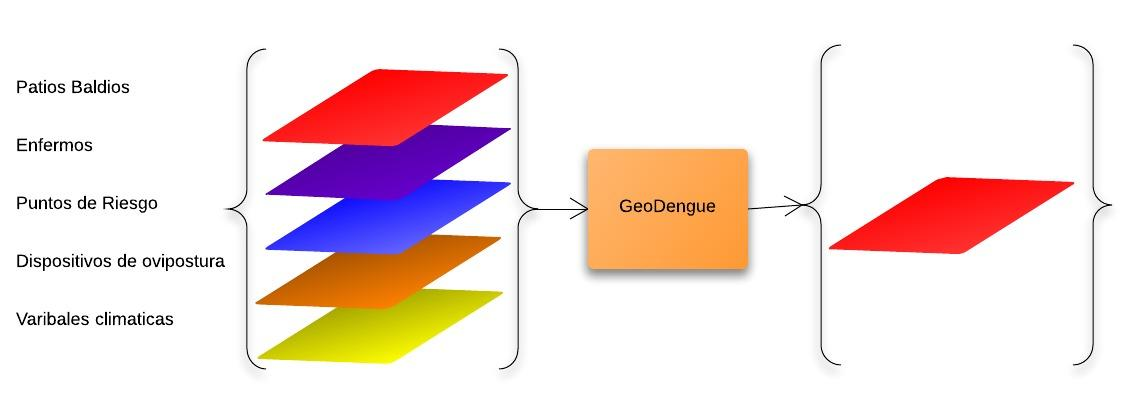
\includegraphics[ scale=0.35]{./graphics/modelo-base.jpeg}
%~ %~
Mediante técnicas de interpolación espacial los datos de entrada serán
procesados y representados en la zona de estudio como polígonos que representan focos de la enfermedad.
%~ %~
Los focos se determina según los valores conocidos de las larvitrampas mediante interpolación, esto representa un instante \cite{AnusuyaSpeech20097}.
 
  %~ * Resultado del conteo de larvas
  %~ * Datos de origen
  %~ * Interpolación
  %~ * Representación
%~ * Predicción de Focos
\section{Proceso Evolutivo}

Se debe explicar lo básico y dar una idea de que se busca y como funciona.


\textbf{Definición 1.} \em Instante \em : Se utiliza el término instante
    para representar a una estrucutra de datos compleja compuesta por
    datos climáticos correspondientes a periodos de tiempos individuales
    $t_{i}$ y otras propiedades complementarias.


\textbf{Definición 2.}\em Peridodo \em : Un periodo es una estrucutra de
    datos que representa a un conjunto de instantes $t_{i}$. El periodo
    $T$ \addsymbol{symbol:P} se define como una colección de $N$ instantes
    $t_{i}$, donde $N$ es el tamaño del periodo de estudio.

    \begin{align*}
        T = t_1,t_2,t_t,\ldots,t_N , & & 1 \leq i \leq N
    \end{align*}


\textbf{Definición 3.} \em Estado \em : Se utliza el término estado
    para representar las etapas del ciclo de desarrollo del \em Aedes Aegypti\em.
    \begin{align*}
        \tau = [huevo, larva, pupa, adulto]
    \end{align*}

\textbf{Definición 4.} \em Sexo \em : Representa el sexo del \em Aedes
    Aegypti\em. Los valores posibles son $MACHO$ y $HEMBRA$.

\textbf{Definición 4.} \em Indiviuduo\em : Se utliza el término individuo
    para representar la unidad del \em Aedes Aegypti \em cualesquiera de sus
    estados, en forma de una estrucutra de datos compleja compuesta de
    propiedades como su madurez y espectativa de vida.

\textbf{Definición 4.} \em Población\em : La población $P$ es una estuctura
    de datos que representa a un grupo de individuos $p_{i}$. Se define como
    una colección de $M$ individuos $p_{i}$, en donde $M$ es el tamaño de
    la población.

    \begin{align*}
        P = p_1,p_2,p_t,\ldots,p_M,  & & 1 \leq i \leq M
    \end{align*}


El proceso evolutivo consiste en somenter los datos, de las muestras obtneidas
mediante la utilización de dispositivos de ovipostura, a las multiples
variaciones climáticas y las caracteristicas biológicas del inividuo.

\section{Consideraciones}
hablar de las consideraciones

Cada $p_{i}$ que pertenzca a $P$ es sometido a las variaciones climáticas de
cada $t_{i}$ que pertenezca a $T$ siempre y cuando $p_{i}$ aún forme parte
de la población $P$.

\section{Operadores básicos}
Durante el proceso evolutivo para cada individuo $p_{j}$ exiten un conjuto
de operadores básicos que son aplicables a todos los individuos sin importar
el sexo y el estado $\tau_{k}$ en el que se encuentre.

hablar de las tablas y la zonificación


\subsection{Madurez}
Para cada $p_{i}$ existe asociado un atributo madurez \addsymbol{symbol:mIi} es
un valor numérico(entre 0 y 100) que varía de acuerdo a las condiciones
climáticas a las que es sometido el mosquito. Cuando la madurez es igual
a 100 el mosquito ya se encuentra listo para un cambio de estado.

\begin{equation}
\eta (t_{i}, p_{j}) = \left\{
  \begin{array}{l l}
    0 & \quad \forall i = 0 \\
    \eta (t_{i-1}, p_{j}) + \frac{1}{\omega(t_{i}) * 24} & \quad \forall i \neq 0
  \end{array} \right.
\end{equation}

\subsection{Cambio de estado}

\begin{equation}
\tau_{k} (t_{i}, p_{j}) = \left\{
  \begin{array}{l l}
    \tau_{k+1} & \quad \forall  \eta(t_{i}, p_{j}) = 100 \\
    \tau_{k} & \quad \text{en caso contrario}
  \end{array} \right.
\end{equation}


\subsection{Mortalidad}
La mortalidad y supervivencia de los individuos se encuentra expresada
mediante la variable de expectativa de vida. La expectativa de vida es
un valor numérico que indica la vitalidad del individuos, esta varía de
acuerdo a las condiciones climáticas a las que es sometido el individuos
durante el proceso evolutivo.

\begin{equation}
\xi (t_{i}, p_{j}) = \left\{
  \begin{array}{l l}
    100 & \quad \forall i = 0 \\
    \xi (t_{i-1}, p_{j}) - \frac{1}{\upsilon(t_{i}) * 24} & \quad \forall i \neq 0
  \end{array} \right.
\end{equation}

El valor de $\xi (t_{i}, p_{j})$ representa el porcentaje de vitalidad del
inidividuo $p_{j}$ luego de ser somenetido a las variaciones del instante
$t_{i}$ perteneciente al periodo $T$ de estudio. La espectativa de vida
para cada individuo $p_{j} \in P$, en el isntante $t_{0}$ se describe como
$\xi (t_{0}, p_{j})= 100$. A medida que $p_{j}$ sea sometido a varios
$t_{i}$ la espectativa de vida irá disminuyendo, si $\xi (t_{i}, p_{j})= 0$ el
idividuo se ha quedado sin espectativa de vida, por lo que se debe proceder
a eliminar $p_{j}$ de $P$ mediante el proceso de reducción de la población
$\theta (t_{i}, p_{j})$.

\begin{equation}
\theta (t_{i}, p_{j}) = \left\{
  \begin{array}{l l}
    p_{j} = null & \quad \xi(t_{i}, p_{j}) == 0 \\
    p_{j} & \quad \text{en caso contrario}
  \end{array} \right.
\end{equation}

\section{Operadores complementarios}
Las etapas inmaduras del \em Aedes Aegigyti\em son principalmente acuaticas
y estaticas, por lo que todas cuentan con caracteristicas similares, no
así la etapa adulto del mosquito que cuenta con ciertas caracteristicas
que divergen mucho del comportamiento básico definido. Debido este
comportamiento especifico todos los $p_{j}$ que se encuentren en el estado
\em Adulto \em cuentan con un conjuto de operadores complementarios que
tienen por objetivo, con ayuda de los operaodres básicos, describir el
comportamiento del mosquito en su estado adulto.

\subsection{Vuelo y búsqueda de alimentos}
Exiten diferencias, en cuanto alimentación y vuelo, entre los adultos
machos y hembras. Los rondan en grupos pequeños o solitariamente,
principalmente atraídos por los mismos huéspedes vertebrados que las hembras.

Las hembras se alimentan principalmente de sangre, que extraen de cualquier
vertebrado, por sus hábitos domésticos muestran marcada predilección por
la del hombre\cite{ThironIzcazaJ2003}. En cuanto a los machos sus partes
bucales no son aptas para chupar sangre, por lo que se alimentan de
carbohidratos de cualquier fuente accesible como frutos o néctar de flores
que satisface sus requerimientos energéticos.

Vuelan en sentido contrario al viento

Por lo general, la hembra de Ae. aegypti no se desplaza más allá de
5,000 m de distancia de radio de vuelo en toda su vida, permanece
físicamente en donde emergió, siempre y cuando no halla algún factor
que la perturbe o no disponga de huéspedes, sitios de reposo y de
postura.


distancia a recorrer
\begin{equation}
 D (t_{i}) = \sqrt{{(\sin(\alpha(t_{i})) * 2000 - S(t_{i}))}^{2}
  + {(\cos(\alpha(t_{i})) * 2000} ^{2} }
\end{equation}
desplazamiento del individuo


\subsection{Reproducción y postura de huevos}



  %~ * Análisis predictivo
  %~ * Descripción del algoritmo de simulación
  %~ * Representación
  %~ * Resultados



\appendix   % inician los apendices de tu tesis

% los cap'itulos que incluyas a partir de aqu'i aparecen
% como ap'endices

% estos comandos generan la bilbiograf'ia
\printbibliography

\end{document}
